
% --------------------------------------------------
% DOCUMENT CLASS
% --------------------------------------------------

\documentclass[
	12pt, 
	]{article}

% --------------------------------------------------
% PACKAGE FILE mypackage.sty
% --------------------------------------------------

%\usepackage{import}
	%\usepackage{package/mypackage}

%\usepackage{packages/mypackage}

% --------------------------------------------------
% DOCUMENT MARGINS:
% --------------------------------------------------

\usepackage[
	a4paper, 
	left   = 2.5cm, 
	right  = 2.5cm,
	top    = 3cm, 
	bottom = 2.5cm
	]{geometry}

% --------------------------------------------------
% INPUT ENCODING:
% --------------------------------------------------

\usepackage[utf8]{inputenc}

% --------------------------------------------------
% FONT ENCODING:
% --------------------------------------------------

\usepackage[T1]{fontenc}

% --------------------------------------------------
% LANGUAGE:
% --------------------------------------------------

\usepackage[
	brazilian,
	english,
	]{babel}

\hyphenation{pa-la-vras pa-ra hi-fe-ni-zar}

% --------------------------------------------------
% FONT:
% --------------------------------------------------

\usepackage{mathpazo}
% \usepackage{palatino} 

% --------------------------------------------------
% PAGE LAYOUT:
% --------------------------------------------------

%\usepackage{fancyhdr}
%\pagestyle{fancy}
%\fancyhead{}
%%\fancyhead[RO,LE]{Section \thesection}
%\fancyfoot{}
%\fancyfoot[R]{\thepage}
%%\fancyfoot[C]{André Luiz Brito}
%\renewcommand{\headrulewidth}{0.0pt}
%\renewcommand{\footrulewidth}{0.0pt}

% --------------------------------------------------
% ENUMERATE INLINE:
% --------------------------------------------------

\usepackage[inline]{enumitem}

% USAGE:
%\begin{enumerate*}[label=(\arabic*)]
%	\item
%	...
%\end{enumerate*}

% --------------------------------------------------
% COLOURS:
% --------------------------------------------------

\usepackage[dvipsnames]{xcolor}

% --------------------------------------------------
% SPACES BETWEEN LINES:
% --------------------------------------------------

\usepackage{setspace}
%\singlespacing
\onehalfspacing
%\doublespacing

% --------------------------------------------------
% PARAGRAPHS:
% --------------------------------------------------

\setlength{\parindent}{1cm}

% --------------------------------------------------
% FIRST PARAGRAPH ALSO 'INDENTED':
% --------------------------------------------------

\usepackage{indentfirst}

% --------------------------------------------------
% SPACES BETWEEN PARAGRAPHS:
% --------------------------------------------------

\setlength{\parskip}{10pt}

% --------------------------------------------------
% SPACE BETWEEN MAIN TEXT AND FOOTNOTES:
% --------------------------------------------------

\setlength{\skip\footins}{1cm}

% --------------------------------------------------
% SPACE BETWEEN FOOTNOTES:
% --------------------------------------------------

\setlength{\footnotesep}{1.5pc}

% --------------------------------------------------
% SPACE BETWEEN FOOTNOTE NUMBER AND TEXT:
% --------------------------------------------------

\usepackage[hang]{footmisc}
\setlength{\footnotemargin}{4mm}

% --------------------------------------------------
% REFERENCES: BIBER
% --------------------------------------------------

\usepackage[
	style        = abnt, %alphabetic, %
	sorting      = nyt, 
	backref      = true, 
	backend      = biber, 
	citecounter  = true, 
	backrefstyle = three, 
	url          = true, 
	maxbibnames  = 99, 
	mincitenames = 1, 
	maxcitenames = 2, 
	hyperref     = true, 
	giveninits   = true, 
	uniquename   = false, 
	uniquelist   = false
	]{biblatex}

\addbibresource{../zip/ref.bib}

% --------------------------------------------------
% IMAGES
% --------------------------------------------------

\usepackage{graphicx}

\graphicspath{ {../images/} }

% --------------------------------------------------
% MULTIFIGURES AND SUBFIGURES
% --------------------------------------------------

\usepackage{caption}
\usepackage{subcaption}


% --------------------------------------------------
% QUOTATION
% --------------------------------------------------

\usepackage{csquotes}

% --------------------------------------------------
% TABLES
% --------------------------------------------------

% new table package:
\usepackage{tabularray}

% commands: \toprule, \midrule, \bottomrule
\usepackage{booktabs}

% Tabelas:
% line break in table cell:
\usepackage{makecell}
% multirow:
\usepackage{multirow}

% long tables:
\usepackage{longtable}

% --------------------------------------------------
% TABLE OF CONTENTS DEPTH:
% --------------------------------------------------

\setcounter{tocdepth}{2}

% --------------------------------------------------
% LIPSUM TEXT
% --------------------------------------------------

\usepackage{lipsum}
\setlipsum{
	par-before = \begingroup\color{gray},
	par-after  = \endgroup
}

% --------------------------------------------------
% MATH ENVIRONMENT
% --------------------------------------------------

\usepackage[
	fleqn % align all equations left
	]{amsmath}

% always after \usepackage{amsmath}:
\usepackage{mathtools}

% --------------------------------------------------
% MATH SYMBOLS
% --------------------------------------------------

\usepackage{amssymb}

% --------------------------------------------------
% NUMBER THE EQUATIONS WITHIN THE SECTION
% --------------------------------------------------

\numberwithin{equation}{section}

% --------------------------------------------------
% SPACE BETWEEN EQUATIONS
% --------------------------------------------------

\setlength{\jot}{5pt}

% --------------------------------------------------
% MATH FONTS
% --------------------------------------------------

% https://ctan.org/pkg/mathalpha?lang=en
\usepackage[
	frak = euler, %boondox, %(for fraktur fonts)
	scr  = cm, %euler, %stixplain, %pxtx, %cm, %zapfc, %(for calligraphic fonts)
	cal  = boondoxo, %boondox, %(for script fonts)
	bb   = bboldx, %pazo, %boondox, %dsfontsans, % (for blackboard bold (double-struck) fonts)
	%bfscr, % force \mathscr to point to the bold version.
	%bfcal, % force \mathcal to point to the bold version.
	%bfbb,  % force \mathbb  to point to the bold version.
	]{mathalpha}

% --------------------------------------------------
% BOLD MATH SYMBOLS
% --------------------------------------------------

% command: \bm{}
\usepackage{bm}

% --------------------------------------------------
% VERBATIM ENVIRONMENT
% --------------------------------------------------

\usepackage{verbatim}
% usage: \begin{verbatim} code \end{verbatim}

% --------------------------------------------------
% MATH COMMANDS
% --------------------------------------------------

% differential d:
\DeclareMathOperator{\dif}{d}

% subject to:
\DeclareMathOperator{\st}{s.t.}

% expectation symbol:
\newcommand{\E}[1][t]{{\mathbb{E}_{#1}}}

% subscript text: $_t$
\newcommand{\subt}[1][t]{{_{#1}}}

% superscript text: $^$
\newcommand{\supt}[1]{{^{#1}}}

% the name of the command:
\newcommand{\com}[1]{\texttt{\textbackslash #1}}

% the greek letter omicron:
\newcommand{\omicron}{o}

% the name of the software:
% \newcommand{\dynare}{\texttt{Dynare}}
\newcommand{\dynare}{\colorbox{lightgray}{$\mathsf{Dynare}$}}
\newcommand{\matlab}{\texttt{MATLAB}}
\newcommand{\octave}{\texttt{OCTAVE}}

% --------------------------------------------------
% CANCEL LINE IN EQUATIONS
% --------------------------------------------------

\usepackage{cancel}
% https://ctan.org/pkg/cancel?lang=en

% --------------------------------------------------
% NICE FRACTIONS INLINE
% --------------------------------------------------

\usepackage{xfrac}

% --------------------------------------------------
% INDEX
% --------------------------------------------------

% USAGE: \index{exemplo}
% options: configure: build: Compile & View | txs:///pdflatex | txs:///makeindex
\usepackage{imakeidx}
\makeindex[intoc] % in table of contents
\indexsetup{othercode=\renewcommand{\indexspace}{\string\textbar\ }}

% --------------------------------------------------
% HYPERTEXT LINKS
% --------------------------------------------------

\usepackage[
colorlinks = true, 
linkcolor  = teal, 
filecolor  = teal, 
urlcolor   = teal, 
citecolor  = teal
]{hyperref}

% --------------------------------------------------
% THEOREMS
% --------------------------------------------------

\usepackage{amsthm}

% DEFINITION:
\theoremstyle{definition}
\newtheorem{definition}{Definition}[section]

% THEOREM:
\theoremstyle{plain}
\newtheorem{theorem}{Theorem}[section]

% LEMMA:
\theoremstyle{plain}
\newtheorem{lemma}{Lemma}[section]

% COROLLARY:
\theoremstyle{plain}
\newtheorem{corollary}{Corollary}[lemma]

% \blacksquare to end the proof:
\renewcommand\qedsymbol{$\blacksquare$}

% --------------------------------------------------
% ACRONYMS
% --------------------------------------------------

\usepackage{acronym} 
% usage: \ac{TLA}

% --------------------------------------------------
% TODO NOTES
% --------------------------------------------------

\setlength{\marginparwidth}{2cm}

\usepackage[
	%disable, % OPTION TO DISABLE THE TODO NOTES.
	textsize = footnotesize,
	color=green!30,
	]{todonotes}

% todo command:
% \todo[inline]{sua tarefa aqui.}

% --------------------------------------------------
% MULTI-FILES PROJECT
% --------------------------------------------------

% best loaded last in the preamble
\usepackage{subfiles}

% --------------------------------------------------
% TITLE
% --------------------------------------------------

% Análise do Impacto da Política Monetária sobre 
% o Produto Interno Bruto Regional: 
% Um Modelo DSGE Regional

\title{
	Analysis of the Monetary Policy Impact \\ 
	on Regional Gross Domestic Product: \\ 
	A Regional DSGE Model \vspace{2cm}}

\author{
	\LARGE André Luiz Brito 
	\footnote{ \href{ 
	mailto:andreluizmtg@gmail.com}{
	andreluizmtg@gmail.com}}}

\date{
	\vfill Curitiba, March 01st, 2023}

% --------------------------------------------------
% DOCUMENT
% --------------------------------------------------

\begin{document}

% --------------------------------------------------
% PRE-TEXT ELEMENTS
% --------------------------------------------------

\maketitle

% no page number:
\thispagestyle{empty}

\newpage

% --------------------------------------------------
% PRE-TEXT ELEMENTS
% --------------------------------------------------

\section*{Pre-text Elements}

\subsection*{Cover Page}

% no page number:
\thispagestyle{empty}

%\newpage

\subsection*{Inside Cover Page}

% no page number:
\thispagestyle{empty}

%\newpage

\subsection*{Cataloging-in-Publication (CIP) data}

% no page number:
\thispagestyle{empty}

%\newpage

\subsection*{Approval Certificate}

% no page number:
\thispagestyle{empty}

%\newpage

\subsection*{Dedication}

% no page number:
\thispagestyle{empty}

%\newpage

\subsection*{Acknowledgments}

% no page number:
\thispagestyle{empty}

%\newpage

\subsection*{Epigraph}

%\null

%\vfill

\begin{flushright}
	
\textit{Neo: I know kung fu. \\
		Morpheus: Show me.}
\end{flushright}

%\vspace{4cm}

% no page number:
\thispagestyle{empty}

\newpage

% --------------------------------------------------
% ABSTRACT
% --------------------------------------------------

{\onehalfspacing
	\begin{abstract}
		\vspace*{0.5cm}
		
		\lipsum[1]
		
\end{abstract}
}

% no page number:
\thispagestyle{empty}

%\newpage

% --------------------------------------------------
% RESUMO
% --------------------------------------------------

{\selectlanguage{brazilian}
	\onehalfspacing
	\begin{abstract}
		\vspace*{0.5cm}
		
		\lipsum[1]
		
\end{abstract}
}

% no page number:
\thispagestyle{empty}

\newpage

% --------------------------------------------------
% LIST OF VARIABLES: ACRONYMS
% --------------------------------------------------

\subsection*{List of Variables}

\begin{acronym}[MPC] % Give the longest label here so that the list is nicely aligned
	\acro{MPC}{model predictive control}
	\acro{TLA}{Three Letter Acronym}
	\acro{uti}[$U$]{utility function}
\end{acronym}

% no page number:
\thispagestyle{empty}

%\newpage

% --------------------------------------------------
% LIST OF ABBREVIATIONS: GLOSSARY
% --------------------------------------------------

\subsection*{List of Abbreviations}

% no page number:
\thispagestyle{empty}

%\newpage

\subsection*{List of Charts} % Lista de Gráficos

% no page number:
\thispagestyle{empty}

%\newpage

\subsection*{List of Figures} % Lista de Quadros

% no page number:
\thispagestyle{empty}

%\newpage

\subsection*{List of Tables} % Lista de Tabelas

% no page number:
\thispagestyle{empty}

%\newpage

\subsection*{List of Abbreviations} % Lista de Abreviações

% no page number:
\thispagestyle{empty}

%\newpage

\subsection*{List of Variables} % Lista de Variáveis

% no page number:
\thispagestyle{empty}

\newpage

% --------------------------------------------------
% TABLE OF CONTENTS
% --------------------------------------------------

\section*{Table of Contents}

{
	\setlength{\parskip}{1pt}
	\singlespacing
	\tableofcontents
}

% no page number:
\thispagestyle{empty}

\newpage

% --------------------------------------------------
% INTRODUCTION
% --------------------------------------------------

\section{Introduction}\label{sec:introduction}

\subfile{section/100_intro}

%\newpage

% --------------------------------------------------
% LITERATURE REVIEW
% --------------------------------------------------

\section{Literature Review}\label{sec:literature-review}

\subfile{section/200_litRev}

\newpage

% --------------------------------------------------
% MODEL
% --------------------------------------------------

\section{Model}\label{sec:model}

\subfile{section/300_model}

\newpage

% --------------------------------------------------
% REGIONS
% --------------------------------------------------

\section{Regions}

\subfile{section/400_regModel}

\newpage

% --------------------------------------------------
% DATA
% --------------------------------------------------

\section{Data}

\lipsum[1]

1. Data Sources

2. Data Treatment

3. Descriptive Statistics

% --------------------------------------------------
% RESULTS
% --------------------------------------------------

\section{Results}

\lipsum[1]

\subsection{Calibration}

% --------------------------------------------------
% PARAMETER CALIBRATION
% --------------------------------------------------

\subsubsection{Parameter Calibration}

\vspace*{-1cm}

\begin{center}
	
	\begin{align}
		\begin{bmatrix}
			\phi       \\
			\varphi    \\
			\sigma     \\
			\beta      \\
			\delta     \\
			\psi       \\
			\theta     \\
			\alpha     \\
			\gamma_R   \\
			\gamma_\pi \\
			\gamma_Y   \\
			\rho_A     \\
			\rho_M     \\
			\theta_C   \\
			\theta_I
		\end{bmatrix} = 
		\begin{bmatrix}
			\phi       \\
			\varphi    \\
			\sigma     \\
			\beta      \\
			\delta     \\
			\psi       \\
			\theta     \\
			\alpha     \\
			\gamma_R   \\
			\gamma_\pi \\
			\gamma_Y   \\
			\rho_A     \\
			\rho_M     \\
			\theta_C   \\
			\theta_I   
		\end{bmatrix}
	\end{align}
	
\end{center}

% --------------------------------------------------
% VARIABLES AT THE STEADY STATE
% --------------------------------------------------

\subsubsection{Variables at the Steady State}

\vspace*{-1cm}

\begin{align}
	\begin{bmatrix}
		P \\
		Z_A \\
		P^\ast \\
		\pi \\
		Z_M \\
		R \\
		\Lambda \\
		W \\
		Y \\
		C \\
		I \\
		K \\
		L
	\end{bmatrix} = 
	\begin{bmatrix}
		P \\
		Z_A \\
		P^\ast \\
		\pi \\
		Z_M \\
		R \\
		\Lambda \\
		W \\
		Y \\
		C \\
		I \\
		K \\
		L
	\end{bmatrix}
\end{align}

\newpage

% --------------------------------------------------
% PARAMETER CALIBRATION
% --------------------------------------------------

\subsubsection{Parameter Calibration}

\vspace*{0.5cm}

\begin{center}
	
\begin{longtblr}[
label = {table:parameter-calibration},
caption = {Parameter Calibration},
remark{Source} = {\cite{costa_junior_understanding_2016}},
]{rowhead = 1,
colspec = {
   Q[c]
  |Q[l]
  |Q[si={table-format=3.2,table-number-alignment=center},c,white]
  }
}
	\hline[2pt]
	\textbf{Parameter} & \textbf{Definition} & \textbf{Calibration} \\ \hline[2pt]
	$\alpha$           & production elasticity with respect to capital & $0.35$ \\ \hline
	$\beta$            & intertemporal discount factor & $0.985$ \\ \hline
	$\gamma_R$         & interest-rate smoothing parameter & $0.79$ \\ \hline
	$\gamma_\pi$       & interest-rate sensitivity in relation to inflation & $2.43$ \\ \hline
	$\gamma_Y$         & interest-rate sensitivity in relation to product & $0.16$ \\ \hline
	$\delta$           & capital depreciation rate & $0.025$ \\ \hline
	$\theta$           & price stickness parameter & $0.8$ \\ \hline
	$\theta_C$         & consumption weight in production  & $0.8$ \\ \hline
	$\theta_I$         & investment weight in production  & $1 -\theta_C$ \\ \hline
	$\rho_A$           & autoregressive parameter of productivity & $0.95$ \\ \hline
	$\rho_M$           & autoregressive parameter of monetary policy & $0.9$ \\ \hline
	$\sigma$           & relative risk aversion coefficient & $2$ \\ \hline
	$\phi$             & relative labor weight in utility & $1$ \\ \hline
	$\varphi$          & marginal disutility of labor supply & $1.5$ \\ \hline
	$\psi$             & elasticity of substitution between intermediate goods & $8$ \\ \hline[2pt]
\end{longtblr}
	
\end{center}

\newpage

% --------------------------------------------------
% VARIABLES AT THE STEADY STATE
% --------------------------------------------------

\subsubsection{Variables at the Steady State}

\vspace*{0.5cm}

\begin{center}
	
\begin{longtblr}[
	label = {table:ss-values},
	caption = {Steady State Values},
	remark{Source} = {\cite{costa_junior_understanding_2016}},
	]{rowhead = 1,
	colspec = {
		Q[c]
		|Q[si={table-format=3.2,table-number-alignment=center},c,white]
			}
		}
		\hline[2pt]
		\textbf{Variable} & \textbf{Steady State Value} \\
		\hline[2pt]
		$P$               & $1$ \\
		\hline
		$Z_A$             & $1$ \\
		\hline
		$P^\ast$          & $1$ \\
		\hline
		$\pi$             & $1$ \\
		\hline
		$Z_M$             & $1$ \\
		\hline
		$R$               & $0.0402$ \\
		\hline
		$\Lambda$         & $0.8750$ \\
		\hline
		$W$               & $1.6967$ \\
		\hline
		$Y$               & $2.6366$ \\
		\hline
		$C$               & $2.1348$ \\
		\hline
		$I$               & $0.5018$ \\
		\hline
		$K$               & $20.0716$ \\
		\hline
		$L$               & $0.8838$ \\
		\hline[2pt]
	\end{longtblr}
	
\end{center}

\newpage

% --------------------------------------------------
% IMPULSE RESPONSE GRAPHICS
% --------------------------------------------------

\subsection{Impulse Response Functions}

\subsubsection{Productivity Shock}

\begin{figure}[h!]
	\centering
\begin{subfigure}[b]{0.3\textwidth}
	\centering
	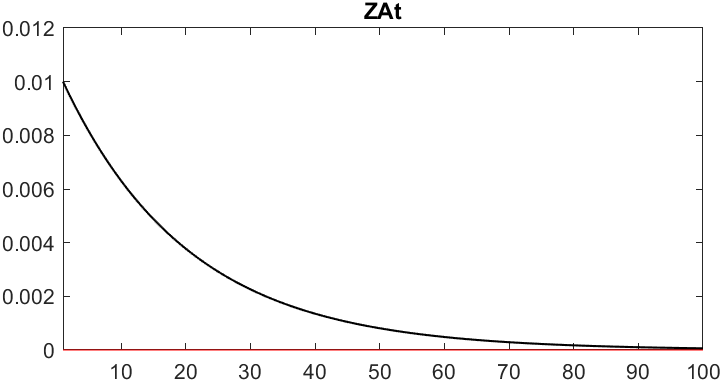
\includegraphics[width=\textwidth]{shock_ZAt/shock_ZAt_ZAt}
	\caption{Productivity Shock}
	\label{fig:zat-productivity-shock}
\end{subfigure}
\hfill
\begin{subfigure}[b]{0.3\textwidth}
	\centering
	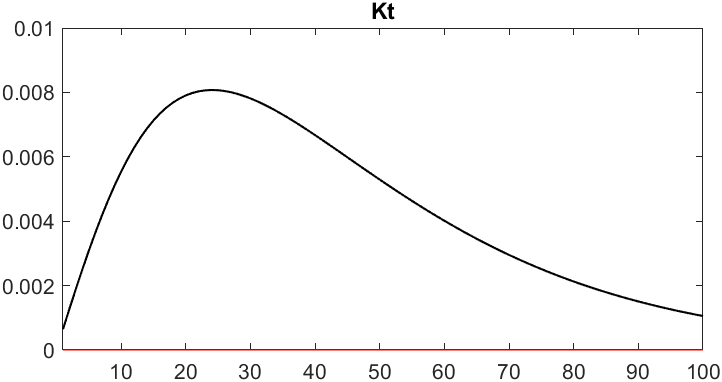
\includegraphics[width=\textwidth]{shock_ZAt/shock_ZAt_Kt}
	\caption{Capital}
	\label{fig:zat-capital}
\end{subfigure}
\hfill
\begin{subfigure}[b]{0.3\textwidth}
	\centering
	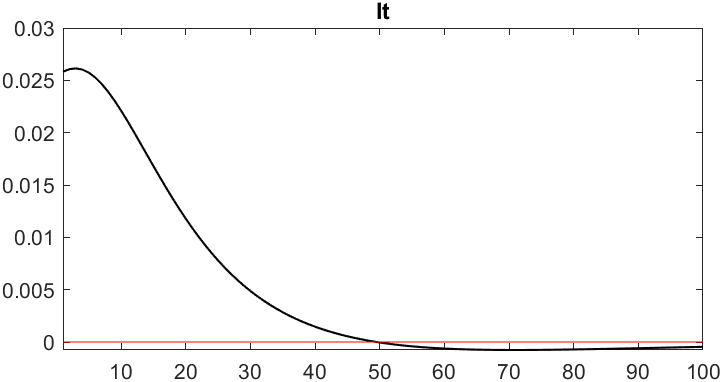
\includegraphics[width=\textwidth]{shock_ZAt/shock_ZAt_It}
	\caption{Investment}
	\label{fig:zat-investment}
\end{subfigure}
\hfill

\vspace*{0.5cm}

\begin{subfigure}[b]{0.3\textwidth}
	\centering
	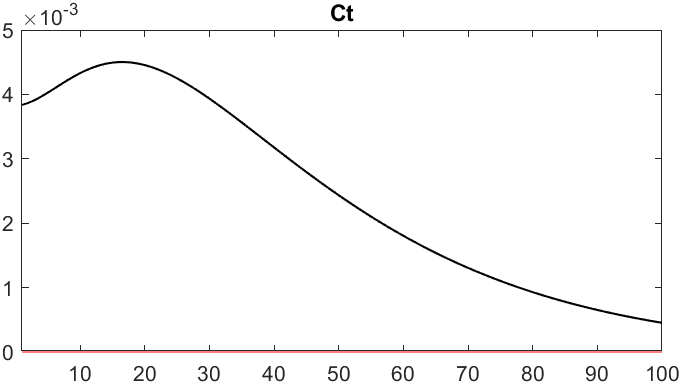
\includegraphics[width=\textwidth]{shock_ZAt/shock_ZAt_Ct}
	\caption{Consumption}
	\label{fig:zat-consumption}
\end{subfigure}
\hfill
\begin{subfigure}[b]{0.3\textwidth}
	\centering
	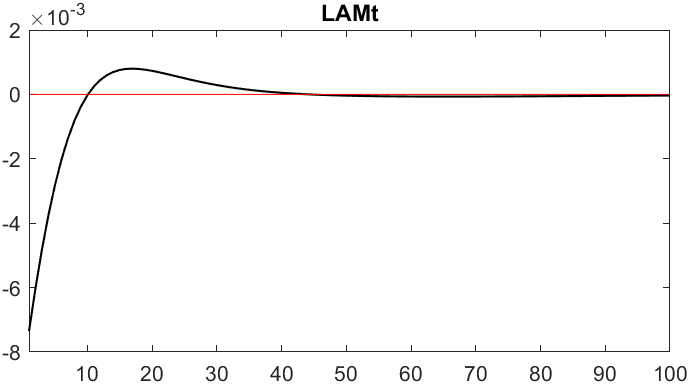
\includegraphics[width=\textwidth]{shock_ZAt/shock_ZAt_LAMBDAt}
	\caption{Marginal Cost}
	\label{fig:zat-marginal-cost}
\end{subfigure}
\hfill
\begin{subfigure}[b]{0.3\textwidth}
	\centering
	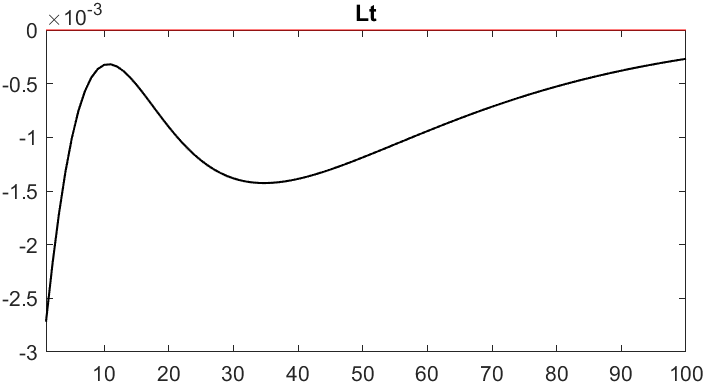
\includegraphics[width=\textwidth]{shock_ZAt/shock_ZAt_Lt}
	\caption{Labor}
	\label{fig:zat-labor}
\end{subfigure}
\hfill

\vspace*{0.5cm}

\begin{subfigure}[b]{0.3\textwidth}
	\centering
	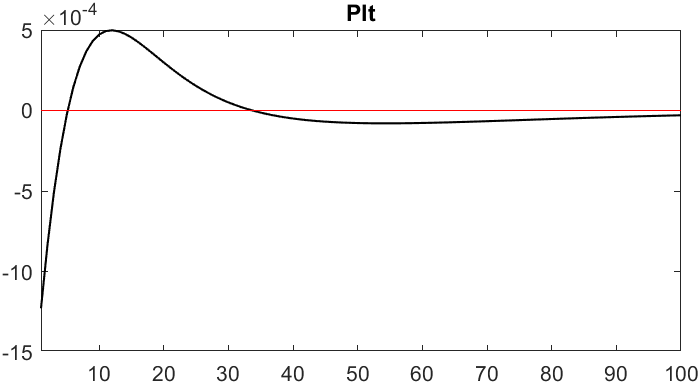
\includegraphics[width=\textwidth]{shock_ZAt/shock_ZAt_PIt}
	\caption{Inflation}
	\label{fig:zat-inflation}
\end{subfigure}
\hfill
\begin{subfigure}[b]{0.3\textwidth}
	\centering
	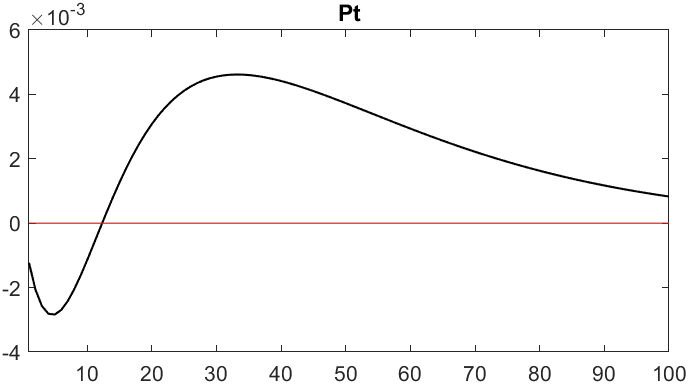
\includegraphics[width=\textwidth]{shock_ZAt/shock_ZAt_Pt}
	\caption{Price Level}
	\label{fig:zat-price}
\end{subfigure}
\hfill
\begin{subfigure}[b]{0.3\textwidth}
	\centering
	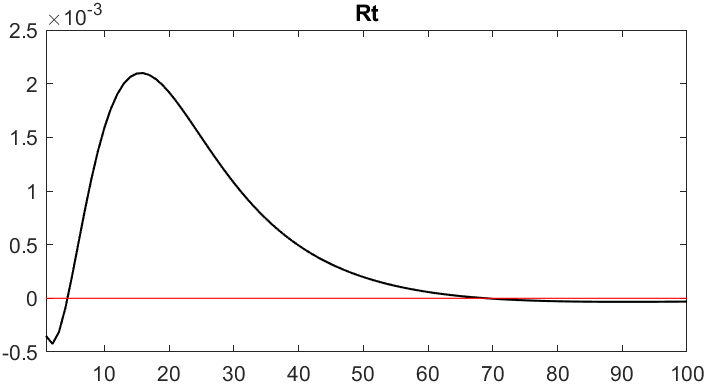
\includegraphics[width=\textwidth]{shock_ZAt/shock_ZAt_Rt}
	\caption{Interest Rate}
	\label{fig:zat-interest-rate}
\end{subfigure}
\hfill

\vspace*{0.5cm}

\begin{subfigure}[b]{0.3\textwidth}
	\centering
	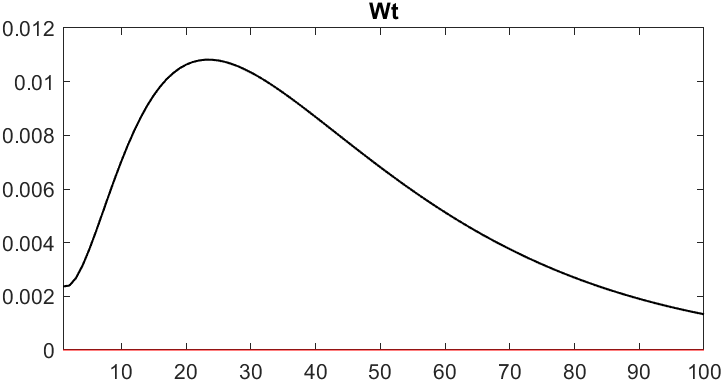
\includegraphics[width=\textwidth]{shock_ZAt/shock_ZAt_Wt}
	\caption{Wage}
	\label{fig:zat-wage}
\end{subfigure}
\hfill
\begin{subfigure}[b]{0.3\textwidth}
	\centering
	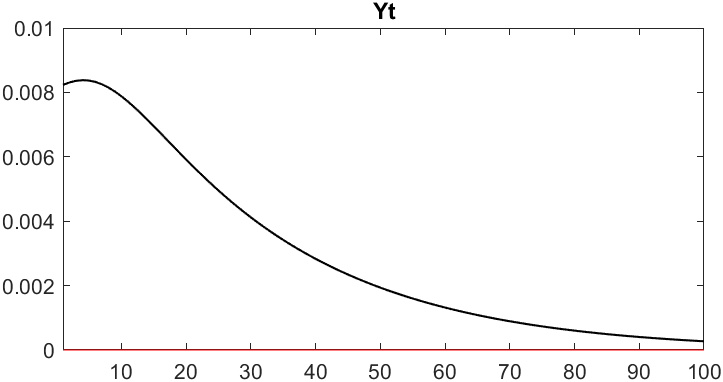
\includegraphics[width=\textwidth]{shock_ZAt/shock_ZAt_Yt}
	\caption{Production}
	\label{fig:zat-production}
\end{subfigure}
\hfill
\begin{subfigure}[b]{0.3\textwidth}
	\centering
	
\includegraphics[width=\textwidth]{shock_ZAt/blank}
\end{subfigure}
\hfill
	\caption{Productivity Shock Impulse Response Functions}
	\label{fig:zat-irf}
\end{figure}

\newpage

\subsubsection{Monetary Shock}

\begin{figure}[h!]
	\centering
	\begin{subfigure}[b]{0.3\textwidth}
		\centering
		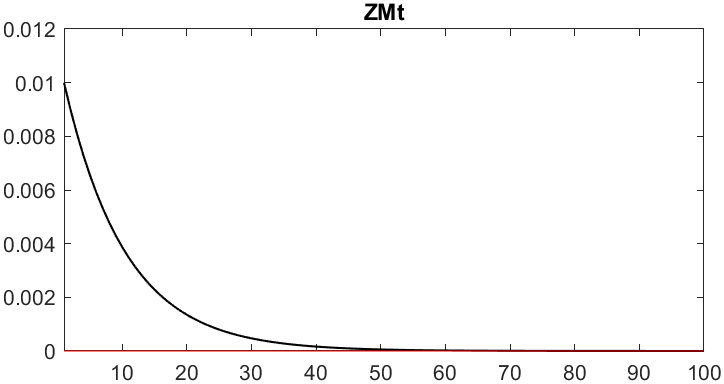
\includegraphics[width=\textwidth]{shock_ZMt/shock_ZMt_ZMt}
		\caption{Monetary Shock}
		\label{fig:ZMt-monetary-shock}
	\end{subfigure}
	\hfill
	\begin{subfigure}[b]{0.3\textwidth}
		\centering
		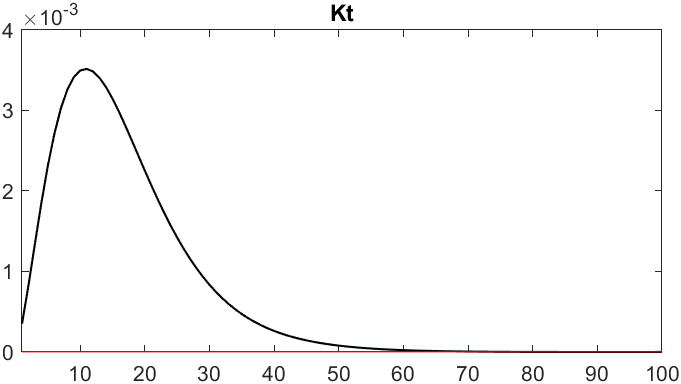
\includegraphics[width=\textwidth]{shock_ZMt/shock_ZMt_Kt}
		\caption{Capital}
		\label{fig:ZMt-capital}
	\end{subfigure}
	\hfill
	\begin{subfigure}[b]{0.3\textwidth}
		\centering
		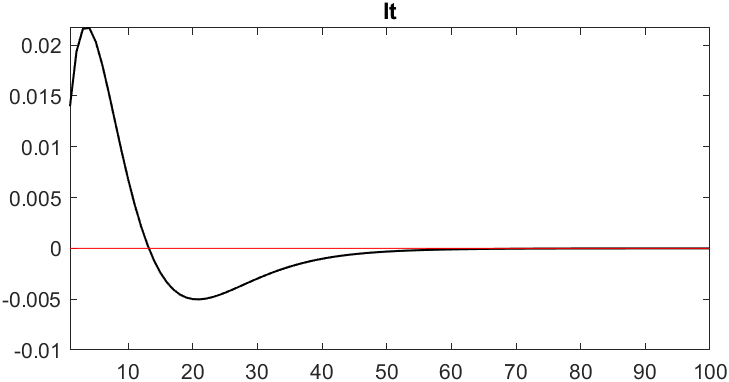
\includegraphics[width=\textwidth]{shock_ZMt/shock_ZMt_It}
		\caption{Investment}
		\label{fig:ZMt-investment}
	\end{subfigure}
	\hfill
	
	\vspace*{0.5cm}
	
	\begin{subfigure}[b]{0.3\textwidth}
		\centering
		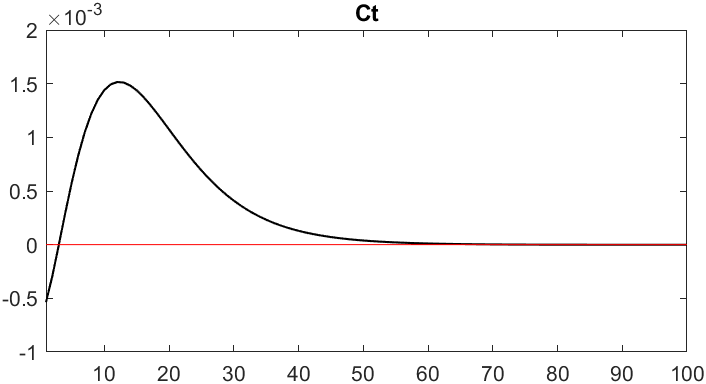
\includegraphics[width=\textwidth]{shock_ZMt/shock_ZMt_Ct}
		\caption{Consumption}
		\label{fig:ZMt-consumption}
	\end{subfigure}
	\hfill
	\begin{subfigure}[b]{0.3\textwidth}
		\centering
		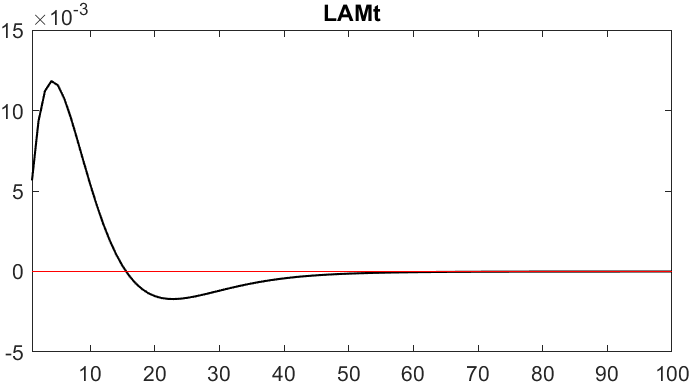
\includegraphics[width=\textwidth]{shock_ZMt/shock_ZMt_LAMBDAt}
		\caption{Marginal Cost}
		\label{fig:ZMt-marginal-cost}
	\end{subfigure}
	\hfill
	\begin{subfigure}[b]{0.3\textwidth}
		\centering
		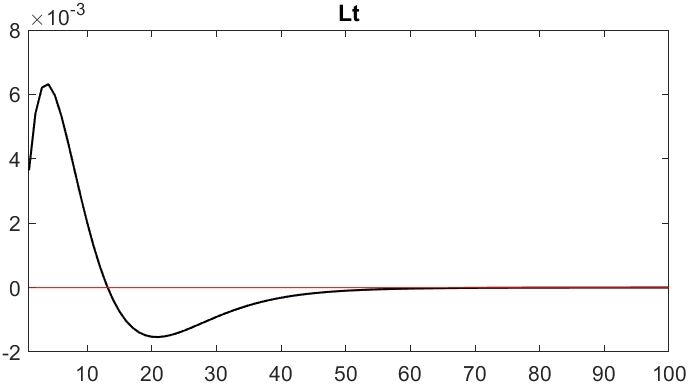
\includegraphics[width=\textwidth]{shock_ZMt/shock_ZMt_Lt}
		\caption{Labor}
		\label{fig:ZMt-labor}
	\end{subfigure}
	\hfill
	
	\vspace*{0.5cm}
	
	\begin{subfigure}[b]{0.3\textwidth}
		\centering
		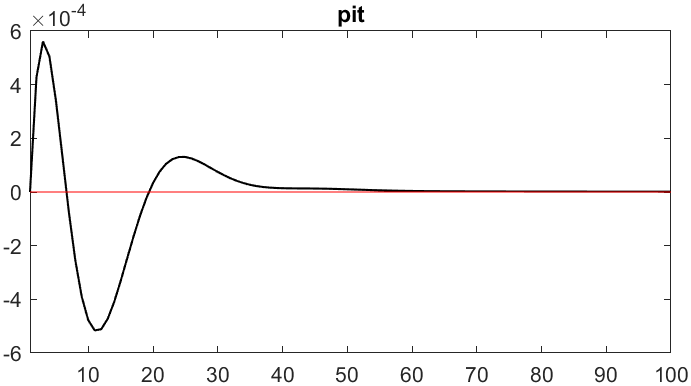
\includegraphics[width=\textwidth]{shock_ZMt/shock_ZMt_PIt}
		\caption{Inflation}
		\label{fig:ZMt-inflation}
	\end{subfigure}
	\hfill
	\begin{subfigure}[b]{0.3\textwidth}
		\centering
		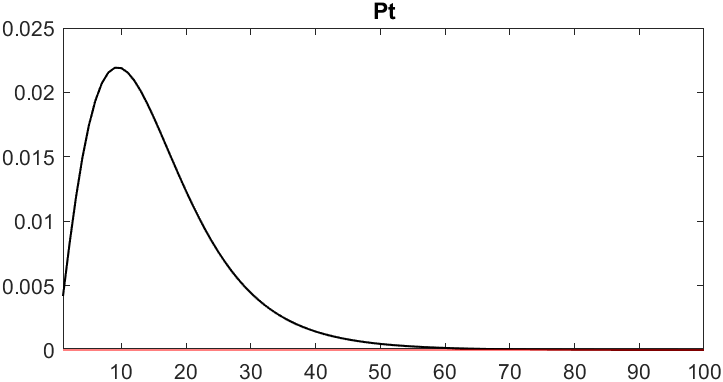
\includegraphics[width=\textwidth]{shock_ZMt/shock_ZMt_Pt}
		\caption{Price Level}
		\label{fig:ZMt-price}
	\end{subfigure}
	\hfill
	\begin{subfigure}[b]{0.3\textwidth}
		\centering
		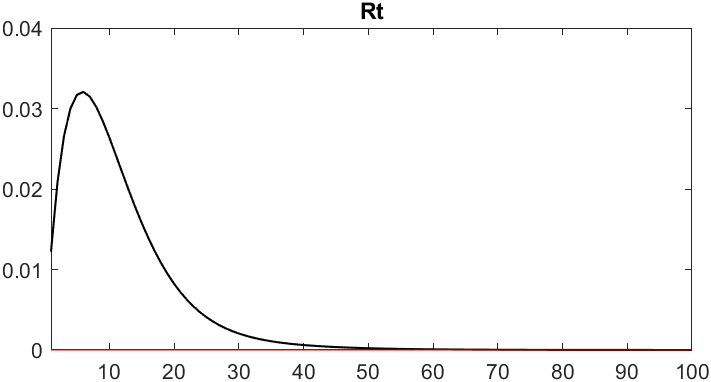
\includegraphics[width=\textwidth]{shock_ZMt/shock_ZMt_Rt}
		\caption{Interest Rate}
		\label{fig:ZMt-interest-rate}
	\end{subfigure}
	\hfill
	
	\vspace*{0.5cm}
	
	\begin{subfigure}[b]{0.3\textwidth}
		\centering
		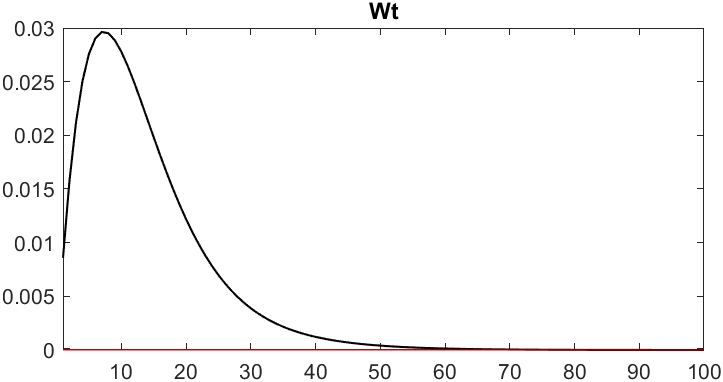
\includegraphics[width=\textwidth]{shock_ZMt/shock_ZMt_Wt}
		\caption{Wage}
		\label{fig:ZMt-wage}
	\end{subfigure}
	\hfill
	\begin{subfigure}[b]{0.3\textwidth}
		\centering
		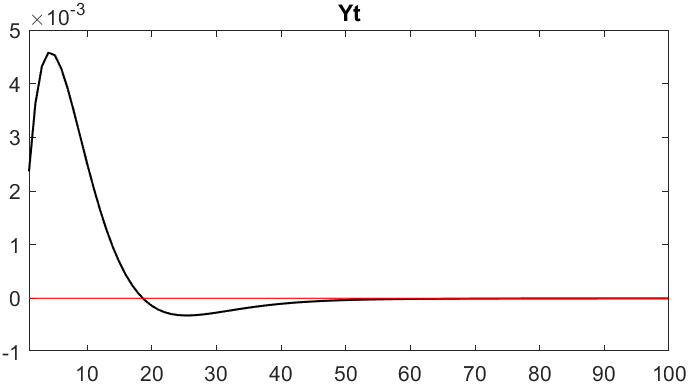
\includegraphics[width=\textwidth]{shock_ZMt/shock_ZMt_Yt}
		\caption{Production}
		\label{fig:ZMt-production}
	\end{subfigure}
	\hfill
	\begin{subfigure}[b]{0.3\textwidth}
		\centering
		
\includegraphics[width=\textwidth]{shock_ZMt/blank}
	\end{subfigure}
	\hfill
	\caption{Monetary Shock Impulse Response Functions}
	\label{fig:ZMt-irf}
\end{figure}

\newpage

\subsection{Parametrization}

\lipsum[1]

% --------------------------------------------------
% FINAL REMARKS
% --------------------------------------------------

\section{Final Remarks}

This section is where you summarize and discuss the main findings, implications, and potential future work related to your research.

\lipsum[1]

\newpage

% --------------------------------------------------
% BIBLIOGRAPHY
% --------------------------------------------------

\section*{Bibliography}

{	
	\onehalfspacing
	\printbibliography[heading=bibintoc]
}

\newpage

% --------------------------------------------------
% APPENDIX
% --------------------------------------------------

\appendix

\subfile{section/900_appendix}

\end{document}